\documentclass[main.tex]{subfiles}

\begin{document}
\section{Performance Results With \starpu}

In order to accurately profile the performance obtained by using the framework, measurements included not only the relevant tests to compare overall execution times with previous approaches, but also tests to analyse the impact of using the framework, and its behaviour in different conditions.

\subsection{Scheduler Impact}

\cref{fig:prof:starpu_cpu} shows the overhead of using the framework to schedule tasks instead of directly invoking them. Execution times were measured with different schedulers, with only \cpu tasks, and compared against the best \cpu times obtained without the framework. No major speedups are expected here, since the framework should itself create a significantly high overhead, but it should be interesting to see if delegating the task of choosing \openmp thread pool size to \starpu, rather than manually tuning it, directly impacts performance.

\image[width=0.6\textwidth]{profiling/starpu_cpu_scheds}{\starpu implementation, \cpu-only}{fig:prof:starpu_cpu}

This was mostly a concern due to the scalability problems observed in \cref{sec:prof:cpu}. If \starpu, using one of the less smart schedulers, would opt to eagerly use all available \cpus, performance would degrade as seen in \cref{fig:prof:cpu}. This was indeed the observed result with the \textbf{peager} scheduler. \textbf{dm} and \textbf{dmda} also degrade performance down to around 4x (which roughly corresponds to worst-case scenarios observed on \cpu implementation), but that is to be expected since these schedulers do not support parallel tasks. Since no accelerators are being used here, this results in all tasks being ran sequentially.

\image[width=0.6\textwidth]{profiling/starpu_cpu_dm_dmda}{\starpu implementation, \cpu sequential vs sequential schedulers}{fig:prof:starpu_cpu_dm_dmda}

Additionally, \cref{fig:prof:starpu_cpu_dm_dmda} shows a comparison of the three sequential versions, namely the framework-less \cpu version with 1 thread, and the \starpu version with the \textbf{dm} and \textbf{dmda} schedulers using only \cpu devices. \textbf{dm} performs slightly worse than \textbf{dmda} in all cases. Since this is a \cpu-only test, it is executed using only the main system memory, so no memory transfers are actually required. The small performance gain from \textbf{dmda} can thus be attributed to the ability of asynchronously allocating requested memory needed in future tasks.


\subsection{Performance with Accelerators}

To test how \gpu devices influenced the algorithm, measurements were made for both individual \gpu, and with both available \gpus for \starpu to use.
When using accelerators, all schedulers are able to speedup the implementation when compared to the best \cpu times (which were achieved with around 6 threads). However, as seen in \cref{fig:prof:starpu_scheds}, the gain difference between each scheduler is noticeable: \textbf{dmda}, which performs poorly on \cpu due to sequentializing tasks sees the largest improvement. This is expected since it is essentially a comparison between sequential \cpu tasks with massively parallel \gpu tasks. The fact to note here is that \textbf{dm} has much worse evolution under the same conditions.
It should be noted here that only a single iteration is being processed at a time. This limits the amount of parallelism available, which results in small performance gains when going from one to two \gpus. The only gain that can be extracted from that is by concurrently executing multiple tasks of the same iteration, one on each device. As seen in \cref{fig:deps}, the number of dependencies is a limiting factor for this.

\begin{figure}[!htp]
  \centering
  \begin{subfigure}{.5\textwidth}
    \centering
    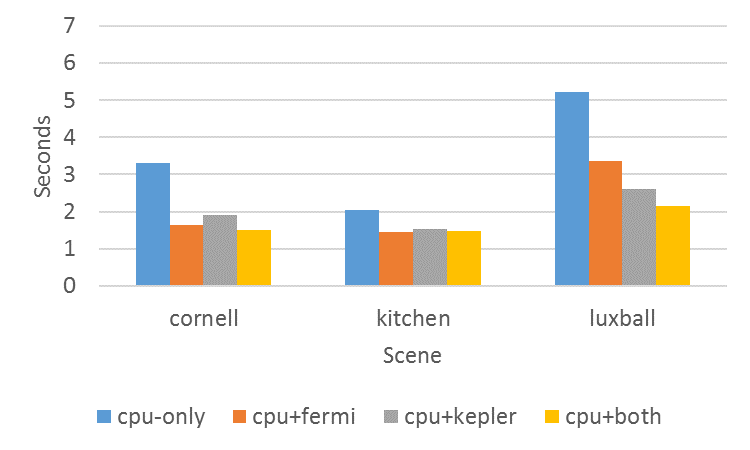
\includegraphics[width=\linewidth]{profiling/starpu_sched_peager}
    \caption{peager \label{fig:prof:starpu_sched_peager}}
  \end{subfigure}%
  \begin{subfigure}{.5\textwidth}
    \centering
    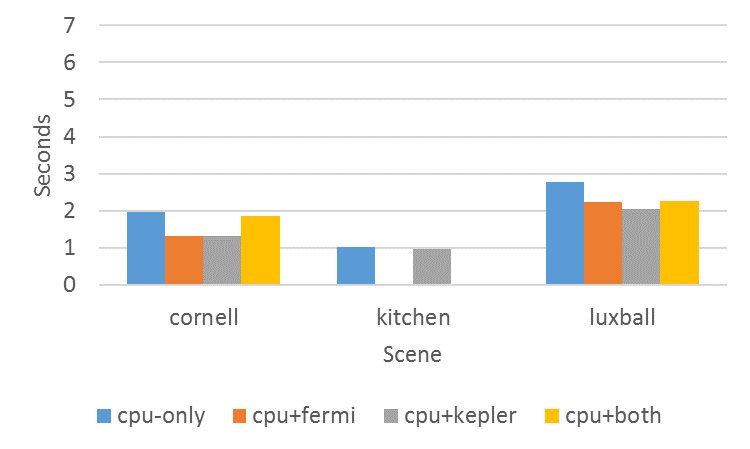
\includegraphics[width=\linewidth]{profiling/starpu_sched_pheft}
    \caption{pheft \label{fig:prof:starpu_sched_pheft}}
  \end{subfigure}
  \begin{subfigure}{.5\textwidth}
    \centering
    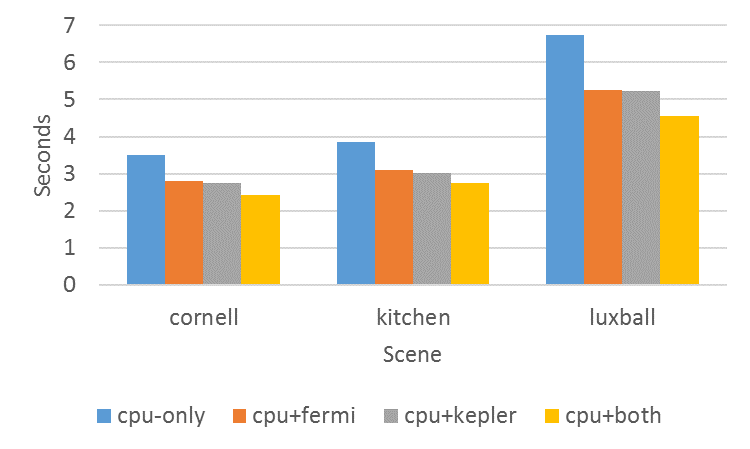
\includegraphics[width=\linewidth]{profiling/starpu_sched_dm}
    \caption{dm \label{fig:prof:starpu_sched_dm}}
  \end{subfigure}%
  \begin{subfigure}{.5\textwidth}
    \centering
    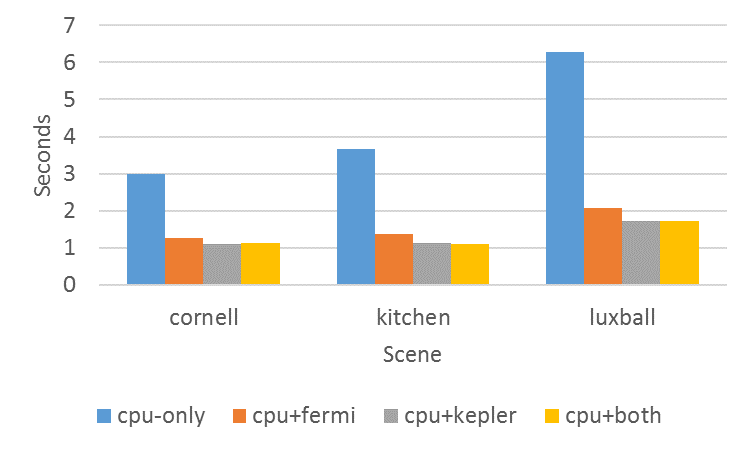
\includegraphics[width=\linewidth]{profiling/starpu_sched_dmda}
    \caption{dmda \label{fig:prof:starpu_sched_dmda}}
  \end{subfigure}
  \caption{Avg. iteration time of the different schedulers with \gpu devices \label{fig:prof:starpu_scheds}}
\end{figure}

This enforces the fact that memory transfers are extremely important to take into account by the scheduler, as this is the only difference between the two.

As for \textbf{peager} and \textbf{pheft}, their gains are not as large, since the \cpu code was already parallelized, but it is relevant to note that the smarter \textbf{pheft} seems to be outperformed once the whole set of devices is used. This is a consequence of the low iteration level-parallelism available. Since each task is fully scheduled to a given device, and multiple task dependencies exist within an iteration, it is difficult to efficiently take advantage of multiple devices simultaneously, in which case eagerly selecting the best device can be considered a faster and more efficient choice.

Unfortunately, when using \textbf{pheft} with the Fermi device, memory errors would constantly be raised, so it was not possible to finish those tests successfully. This is most likely due to problems with this particular scheduler, which is still under development by the \starpu team, and thus cannot be assumed to be fully functional.


\subsection{Calibration} \label{sec:prof:calibration}

\starpu builds a performance model for each task by calibrating them on the first executions. Once 10 executions are profiled, calibration is finished for that task and the performance model can start to be used. \Cref{fig:prof:starpu_calibrate} shows how calibration affects each scheduler. Each case consists of running 100 iterations of the algorithm with no performance model to start with (deleted prior to the execution). This performance model is then build in the initial stages of the algorithm, until a good amount of sampling is obtained (at least 10 executions for each different task on each different device).
Results show very different behaviours between schedulers.

\textbf{peager}, being a more naive algorithm, does not actually perform calibration, and does not seem to evolve very efficiently. A drop in execution time can be seen across time, but since all devices are eagerly used whenever possible, this results in more workload being assigned to the \cpus, which have worse performance when compared to gpus, as explained in previous sections. It should also be noted that \textbf{peager} was found to always employ 14 \openmp threads for each task, assigning it all available cores. This is not the best choice, as it was noted in \cref{sec:prof:cpu} that tasks do not scale beyond 6 threads. The apparent drop in \cpu time that can be observed in \cref{fig:prof:starpu_calibrate_peager} is not due to better thread pool size selection, but rather the result of more tasks being offloaded to \gpus.

\begin{figure}[!htp]
  \centering
  \begin{subfigure}{.5\textwidth}
    \centering
    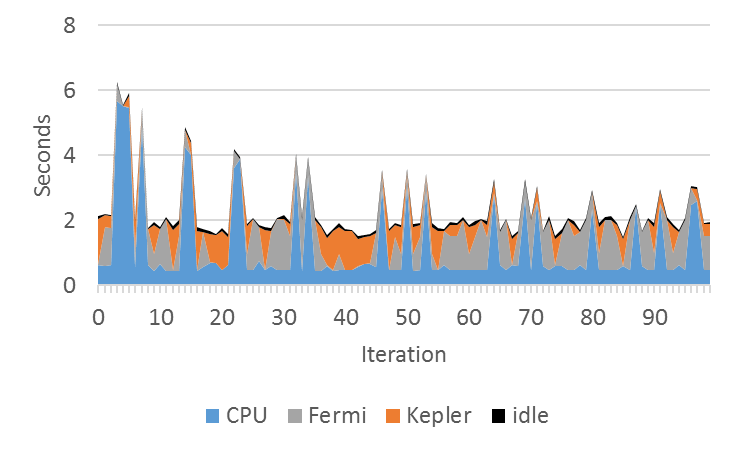
\includegraphics[width=\linewidth]{profiling/starpu_calibrate_peager}
    \caption{peager \label{fig:prof:starpu_calibrate_peager}}
  \end{subfigure}%
  \begin{subfigure}{.5\textwidth}
    \centering
    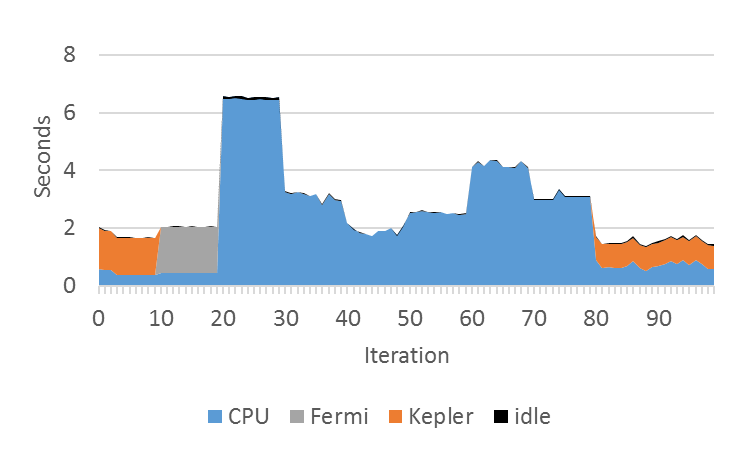
\includegraphics[width=\linewidth]{profiling/starpu_calibrate_pheft}
    \caption{pheft \label{fig:prof:starpu_calibrate_pheft}}
  \end{subfigure}
  \begin{subfigure}{.5\textwidth}
    \centering
    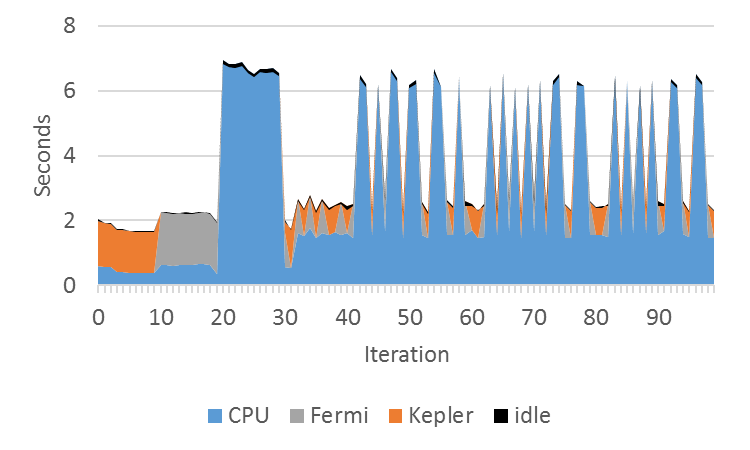
\includegraphics[width=\linewidth]{profiling/starpu_calibrate_dm}
    \caption{dm \label{fig:prof:starpu_calibrate_dm}}
  \end{subfigure}%
  \begin{subfigure}{.5\textwidth}
    \centering
    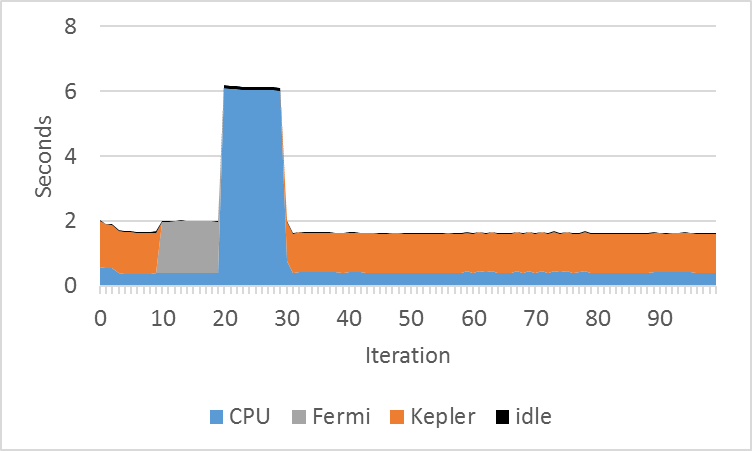
\includegraphics[width=\linewidth]{profiling/starpu_calibrate_dmda}
    \caption{dmda \label{fig:prof:starpu_calibrate_dmda}}
  \end{subfigure}
  \caption{Calibration process starting with an empty performance model \label{fig:prof:starpu_calibrate}}
\end{figure}

For the remaining schedulers, calibration can be clearly noticed in the first 30 iterations of each one. Each calibration starts by running 10 iterations almost entirely on the Kepler device (an entire iteration would not be possible, since some tasks are \cpu-only), following the Fermi device, and finally the \cpu devices.

After the initial calibration, \textbf{pheft} continues to calibrate the \cpu implementation, by successfully choosing different thread pool sizes, until the best one is found. After this process, the initial calibration is finished, and the scheduler progresses normally.

\textbf{Dm} and \textbf{dmda} do not support combined workers, so \cpu calibration is restricted to using only 1 \cpu thread at a time. Since \textbf{dmda} is a data-aware version of the original \textbf{dm}, it deals more efficiently with data transfers. This being the only difference, \textbf{dmda} seems to perform much better, offloading most computations to the Kepler device, while \textbf{dm} still runs some iterations on the \cpu. This is a result of \textbf{dm} not being able to asynchronously perform required data transfers, thus \gpu task execution costs (including the required communication) are much higher, ending up with a significant part of it being kept on the \cpu.



\subsection{Overall Performance Comparison}

The best case scenario for each approach is shown in \cref{fig:prof:overall}. This serves to show the impact of \starpu with each different scheduler against framework-less solutions.

\begin{figure}[!htp]
  \centering
  \begin{subfigure}{.5\textwidth}
    \centering
    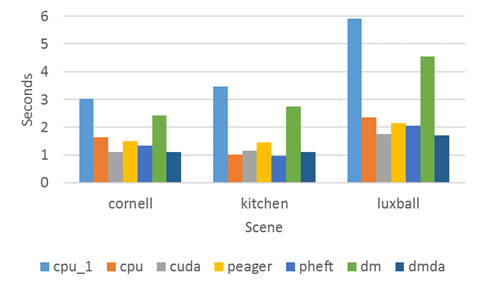
\includegraphics[width=\linewidth]{profiling/1iter_time}
    \caption{Avg. iteration time \label{fig:prof:overall_time}}
  \end{subfigure}%
  \begin{subfigure}{.5\textwidth}
    \centering
    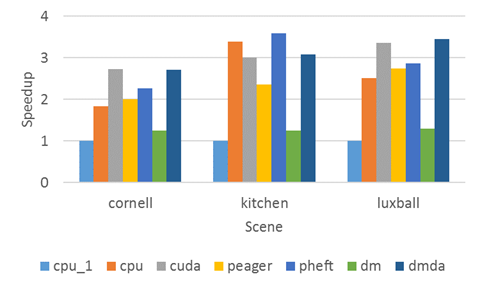
\includegraphics[width=\linewidth]{profiling/1iter_speedup}
    \caption{Speedup \label{fig:prof:overall_speedup}}
  \end{subfigure}
  \caption{Best cases for each different implementation and scheduler \label{fig:prof:overall}}
\end{figure}

\begin{table}[!htb]
  \begin{tabular}{|r|rrr|rrrr|}
    \hline
            & Sequential & \cpu & \gpu & \textbf{peager} & \textbf{pheft} & \textbf{dm} & \textbf{dmda} \\ \hline
    cornell & 3.03       & 1.65 & 1.11  & 1.51            & 1.33           & 2.42        & 1.12 \\
    kitchen & 3.46       & 1.02 & 1.15  & 1.46            & 0.96           & 2.75        & 1.12 \\
    luxball & 5.91       & 2.35 & 1.76  & 2.15            & 2.06           & 4.55        & 1.71 \\
    \hline
  \end{tabular}
  \caption{Avg Iteration time for all versions \label{tab:overall_time}}
\end{table}

\begin{table}[!htb]
  \begin{tabular}{|r|rr|rrrr|}
    \hline
            & \cpu & \gpu & \textbf{peager} & \textbf{pheft} & \textbf{dm} & \textbf{dmda} \\ \hline
    cornell & 1.83 & 2.73  & 2.01            & 2.27           & 1.25        & 2.71 \\
    kitchen & 3.39 & 2.30  & 2.36            & 3.60           & 1.26        & 3.09 \\
    luxball & 2.52 & 3.36  & 2.75            & 2.87           & 1.30        & 3.45 \\
    \hline
  \end{tabular}
  \caption{Avg speedup for all versions \label{tab:overall_speedup}}
\end{table}

\subsection{Concurrent Iterations}

With the employed approach, task-level parallelism is limited. The \textbf{dmda} does not support combined workers, greatly lowering efficiency of \cpu tasks. \textbf{pheft} does support this, but its not a data aware scheduler, meaning that data transfers are not considered when assigning tasks. As a result, performance with \starpu is limited when using processing a single iteration. The attempted solution was to allow the execution of a variable number of concurrent iterations, in order to take advantage of multiple devices without the limitation of dependencies. Results shown in \

\image[width=0.6\textwidth]{profiling/iters_at_once_both_speedup}{Speedup with concurrent iterations}{fig:prof:iters_at_once_both_speedup}

Results show in \cref{fig:prof:iters_at_once_both_speedup} indicate this was not a successful approach, as the best speedup achieved was slightly above 2, when using between 16 to 32 concurrent iterations. Further analysis of the results indicated that when using this approach, large contention points appeared at the end of each iteration, which consists of 2 computational tasks that have to be ran sequentially on \cpu (see \cref{fig:diagram_cpu}). These tasks essentially perform memory operations, to aggregate the result of the individual iteration into the final aggregated image. This works as a barrier, since two iterations cannot be merged concurrently to the final image, slowing all iterations in that stage.

One possible alternative that could be attempted to seek better results was an approach based on data partitioning rather than concurrent iterations. Since multiple iterations seem to create excessive memory contention, partitioning data using the \starpu API, and manually defining task granularity might be an alternative way to extract more parallelism from a single iteration, since each sub task can be assigned to different devices.

\end{document}
